\documentclass[9pt]{beamer}

%~~~~~~~~~~~~~~~~~~~~~~~~~~~~~~~~~~~~~~~~~~~~~~~~~~~~~~~~~~~~~~~~~~~~~~~~~~~~~~
% Use roboto Font (recommended)
\usepackage[sfdefault]{roboto}
\usepackage[utf8]{inputenc}
\usepackage[T1]{fontenc}
%~~~~~~~~~~~~~~~~~~~~~~~~~~~~~~~~~~~~~~~~~~~~~~~~~~~~~~~~~~~~~~~~~~~~~~~~~~~~~~

%~~~~~~~~~~~~~~~~~~~~~~~~~~~~~~~~~~~~~~~~~~~~~~~~~~~~~~~~~~~~~~~~~~~~~~~~~~~~~~
% Define where theme files are located. ('/styles')
\usepackage{styles/fluxmacros}
\usefolder{styles}
% Use Flux theme v0.1 beta
% Available style: asphalt, blue, red, green, gray 
\usetheme[style=asphalt]{flux}
%~~~~~~~~~~~~~~~~~~~~~~~~~~~~~~~~~~~~~~~~~~~~~~~~~~~~~~~~~~~~~~~~~~~~~~~~~~~~~~

%~~~~~~~~~~~~~~~~~~~~~~~~~~~~~~~~~~~~~~~~~~~~~~~~~~~~~~~~~~~~~~~~~~~~~~~~~~~~~~
% Extra packages for the demo:
\usepackage{booktabs}
\usepackage{colortbl}
\usepackage{ragged2e}
\usepackage{schemabloc}
%~~~~~~~~~~~~~~~~~~~~~~~~~~~~~~~~~~~~~~~~~~~~~~~~~~~~~~~~~~~~~~~~~~~~~~~~~~~~~~

%~~~~~~~~~~~~~~~~~~~~~~~~~~~~~~~~~~~~~~~~~~~~~~~~~~~~~~~~~~~~~~~~~~~~~~~~~~~~~~
% Informations
\title{Computación distribuida.}
\subtitle{Aplicaciones de Relojes Vectoriales.}
\author{Integrantes:\\
        Aguilera Moreno Adrian\\
        Torres Valencia Kevin Jair\\
        Pérez Romero Natalia Abigail}
\institute{Facultad de Ciencias, UNAM}
\date{\today}
\titlegraphic{Imagenes/im1.png}
%~~~~~~~~~~~~~~~~~~~~~~~~~~~~~~~~~~~~~~~~~~~~~~~~~~~~~~~~~~~~~~~~~~~~~~~~~~~~~~

\begin{document}

% Generate title page
\titlepage

\begin{frame}
 \frametitle{Tabla de contenido.}
 \tableofcontents
\end{frame}

\section{Presentation}

\subsection{introduction}

%%%%%%%%%%%%%%%%%%% Pruebas
\begin{frame}{Flux}{introduction}
	\justifying
 Flux is a modern style beamer presentation. It is provided as a work in progress version and may suffer from inconsistencies. Sources and complementary information are available at\\[0.3cm]
 	\centering\textbf{github.com/pvanberg/flux-beamer}
\end{frame}


\def\beamer@mytheme@style{green}
%%%%%%%%%%% Aquí va la solución al problema 1.
\newpage
\textbf{\textcolor{MidnightBlue}{1.}} Considera la siguiente variante del algoritmo
de consenso con terminación temprana.
Contesta lo siguiente:
\begin{enumerate}[a)]
    \item Demuestra que el algoritmo 1 soluciona el problema del consenso,
    tolerando $f < n$ fallas de tipo paro, donde $n$ es el número de procesos en el sistema.

    Por demostrar:
    \begin{itemize}
        \item Terminación

        El algoritmo no tiene una clara condición de salida. La linea 6 se
        ejecutara indefinidamente, a menos que exista una en la linea 9 cuando
        se ejecuta \textit{decide max(vista)}.

        \item Validez

        El valor de \textit{prop = vista} fue propuesto por algún proceso en cada ronda.

        \item Acuerdo.
        No queda claro si el algoritmo termina, sin embargo:
        Veamos una ejecución cuando $f=0$:
        Al inicio de la ejecución $r=0$, la \textit{flag = false},
        envía $<prop,false>$, luego $r=1$,
        $vista = prop, prop_1$, luego
        $rec[1]= 1+1$ y no se modifica \textit{flag}
        hasta que $rec[1-1]==rec[1]$,
        en esta ronda no se modifica \textit{flag}


        Cuando $r=2$,
        $send(<prop_2,false>)$ a todos
        \textit{vista = \{$prop,prop_1,prop_2$\}}
        $rec[2]=1+1$

        $rec[2-1]==rec[2] \rightarrow rec[1]==rec[2]$, en esta ronda se modifica $flag=true$


        Cuando $r=3$,
        $send(<prop_2,true>)$ a todos
        \textit{decide max(vista)}
        \textit{vista = \{$prop,prop_1,prop_2,prop_3$\}}
        \textit{ dec = true}
        $rec[3]=1+3$
        $rec[3-1]==rec[3] \rightarrow rec[2]==rec[3]$, en esta ronda no se modifica $flag=true$


        Cuando $r=4$,
        $send(<prop_3,true>)$ a todos
        \textit{decide max(vista)}
        \textit{vista = \{$prop,prop_1,prop_2,prop_3,prop_4$\}}
        \textit{dec = true}
        $rec[4]=1+3$

        $rec[4-1]==rec[4] \rightarrow rec[3]==rec[4]$, en esta ronda no se modifica $flag=true$

        Si algún proceso tuviera una falla de tipo paro, el valor de vista sería
        diferente y si al menos una flag de la ronda anterior es verdadera entonces
        llega a un acuerdo con los valores de vista. Por lo tanto en cada dos
        rondas a partir de la tercera, todos los proceso (vivos) acuerdan el mismo valor.
    \end{itemize}


    \item ¿Es cierto que los procesos correcto terminan en a lo más
    $max(t +2, f +1)$ rondas en el algoritmo 1? Argumenta tu respuesta.
    Recuerda que $t \leq f$ es el número de fallas que realmente ocurren en una
    ejecución dada.\\
    Si $t$ es el número de fallas que realmente ocurren en una ejecución y $f$ es el número de fallas de tipo paro.
    Notemos que el algoritmo toma dos rondas para poder llegar a consenso: en la primer ronda recibe los mensajes y los almacena en la variable $vista$ por la linea 10. Aplicar $or$ a las flags que al momento son $false$, y luego al verificar $rec[r-1]==rec[r]$ y actualice $flag=true$. Para que en la segunda ronda decida el $max$ a partir de $vista$, la cual es la union de las vistas propuestas por los procesos en la ronda uno. 
    
    De manera similar al algoritmo del consenso visto en clase se tardara $t+1$ rondas en llegar a un consenso pero notemos que si encontramos un error más de los esperados son necesarias dos rondas más para llegar a un consenso.

    \item Haz un análisis del número máximo de mensajes que se envían en una
    ejecución del algoritmo 1. Tu cota debe estar en función de $n$ y $f$.

    El número de mensajes máximo se puede expresar como la suma de todos los mensajes recibidos por cada proceso en cada ronda, lo cual es almacenado en cada ronda en la variable \textit{rec[r]} en la linea 14
    \[\sum_{i=0}^r rec[i] = 1+rec[0]+1+rec[1]\]
\end{enumerate}

\begin{figure}
    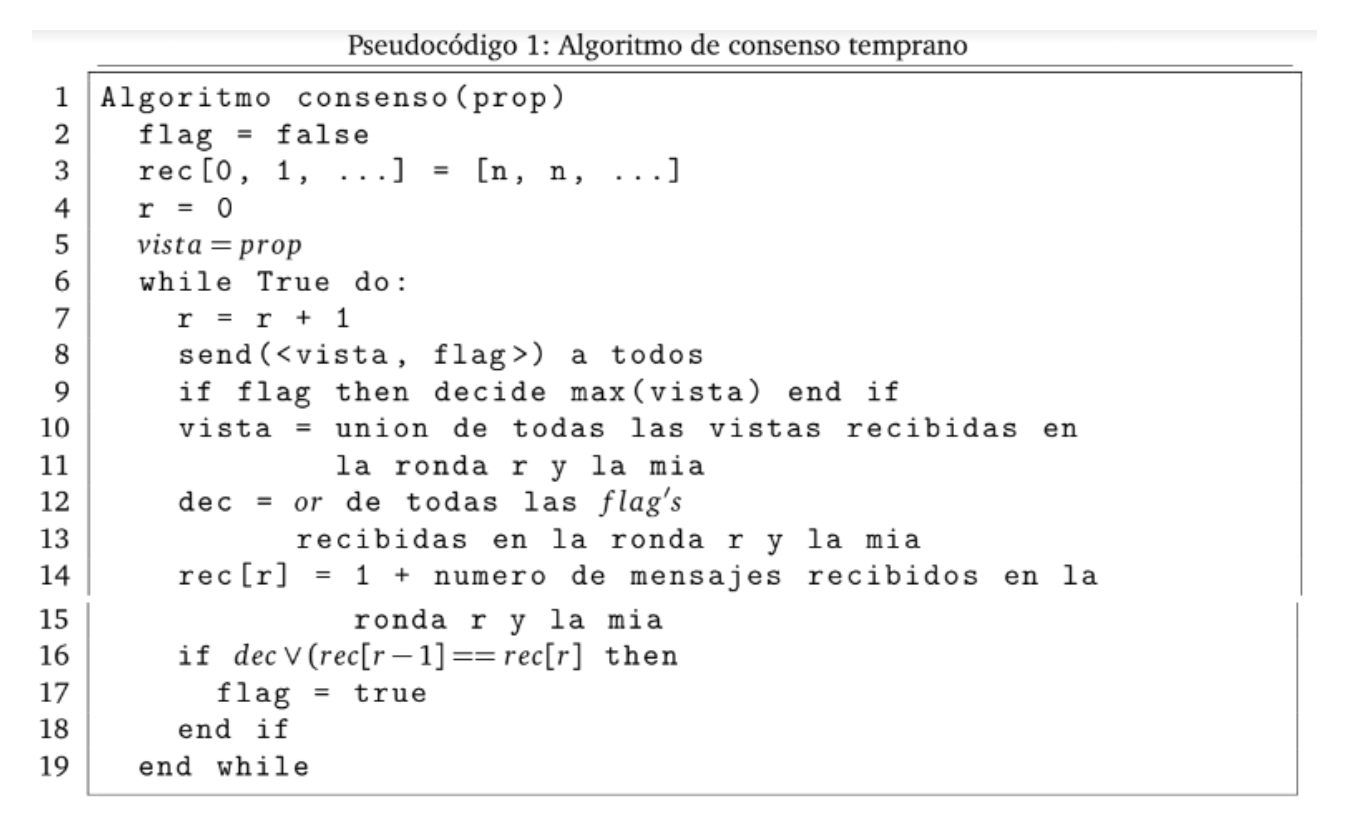
\includegraphics[width=\textwidth]{consensoTemprano.png}
\end{figure}


\subsection{fonts}
%%%%%%%%%%% Aquí va la solución al problema 1.
\newpage
2. Retomando el problema de los dos enamorados con
los mismos requerimientos vistos en clase, responda
las siguientes preguntas:

\begin{itemize}
\item Suponga que las citas sólo se pueden realizar
  entre las 21:00 y las 22:00 horas. ¿Tiene solución
  el problema en este caso?
  
  El problema no tiene solución, porque a pesar de que el intervalo de tiempo en que la cita puede se realizada se vio reducido, persiste el problema de no poder reconocer cuando un mensaje ya ha sido entregado o se perdió, de manera que aún no es posible que los enamorados puedan ponerse de acuerdo para su cita.

\item ¿El problema tiene solución cuando añade el siguiente
  requerimiento: los amantes deben ser capaces de coordinar
  una hora para una cita solamente cuando ningún mensaje
  se pierde, y, en cualquier otro caso, ellos no deberían
  presentarse?
  
 El problema no tiene solución, la imposibilidad es justo igual a la del problema original. Los enamorados no pueden saber si su mensaje ha sido recibido y deben presentarse a la cita.  

\item Consideremos una variación: Los dos amantes se han
  cuenta de que no necesitan ponerse de acuerdo sobre una
  hora exacta para la reunión, está bien si sus horas de
  reunión son lo suficientemente cercanas. En otras palabras,
  cada uno debería eventualmente elegir un tiempo, de modo
  que los dos tiempos estén lo suficientemente cerca. ¿Se
  puede resolver su problema?
  
  No, el problema no tiene solución. Porque es poco probable que dos intervalos sobre un periodo de tiempo indeterminado coincidan, además de que persiste el problema de indistinguibilidad, de forma que los enamorados tienen la incertidumbre si su mensaje fue recibido o no.
  
\end{itemize}


\subsection{footnotes}
\newline
\textbf{\textcolor{MidnightBlue}{3.}}
Supongamos que no tenemos suficientes recursos para equipar todas nuestras máquinas
con detectores de fallos. En su lugar, ordenamos detectores de fallos eventualmente
fuertes para $k$ máquinas y las restantes $n-k$ máquinas tienen detectores de fallos
fake que nunca sospechan de nadie. La elección de cuales máquinas obtienen el
detector 
de fallos real y cuales obtienen los falsos, está bajo el control de un adversario.

Esto significa que todo proceso fallido es eventualmente puesto bajo sospecha de
manera permanente por todo procesos no fallido con un detector de fallos real, y hay
al menos un proceso no fallido que eventualmente no es puesto bajo sospecha de forma
permanente por nadie. Llamemos al detector de fallas resultante $\Diamond S_k$.\\

Sea $f$ el número actual de fallas. ¿Bajo que condiciones de $f$, $k$ y $n$ se puede
resolver el consenso en el modelo usual de paso de mensajes asíncrono determinista
usando $\Diamond S_k$?\\



\section{Collections}

\subsection{lists}
%%%%%%%%%%% Aquí va la solución al problema 4.
\newpage
\textbf{\textcolor{MidnightBlue}{4.}} Considera el algoritmo 1,
que calcula una $\Delta + 1$ coloración, donde $\Delta$ es el
grado máximo en la gráfica. Muestra una gráfica $G$ con al menos
10 vértices y una asignación de IDs, donde el algoritmo coloree
todos los procesos (el primer momento en el que todas las variables
$c$ son distintas de $\bot$) en tiempo $diam(G)$. Muestra otra
asignación de IDs para las que el algoritmo coloree en tiempo a los
más $diam(G)/2$.

\begin{figure}[ht]
        \begin{center}
                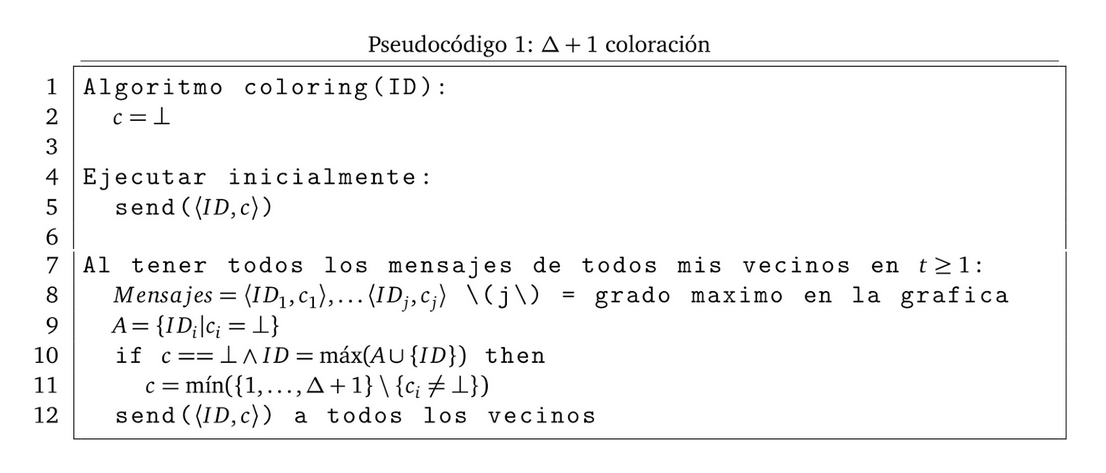
\includegraphics[width=15cm]{AlgoritmoP5.png}
        \end{center}
\end{figure}

$\rhd$ Para este problema dividamos la solución en $3$ respectivas
soluciones:                                                             \newline

\hspace*{0.5cm} \textbf{\textcolor{blue}{1}}. Mostrar una ejecución
en tiempo \code{diam($G$)}, con $G$ una gráfica tal que $|V_G| = 10$.

\begin{figure}[ht!]
     \centering
     \begin{tikzpicture}
        \begin{scope}
           % Fig exterior:
           \node(0) [vertex, label=180:$p_0$] at (-2, 0)       {};
           \node(1) [vertex, label=180:$p_1$] at (2,  0)       {};
           \node(2) [vertex, label=180:$p_2$] at (3.24, 3.81)  {};
           \node(3) [vertex, label=180:$p_3$] at (0, 6)        {};
           \node(4) [vertex, label=180:$p_2$] at (-3.24, 3.81) {};
           % Fig interior:
           
           
           \node (L) at (-5,5){$G$};
        \end{scope}
     \end{tikzpicture}
\caption{Gŕagica $G$.}
\label{fig:fam1}
\end{figure}

\hfill $\lhd$


\subsection{tables}
%%%%%%%%%%% Aquí va la solución al problema 5.
\newpage
\textbf{\textcolor{MidnightBlue}{5.}} El algoritmo puede mejorar su complejidad de tiempo si se ejecutan de forma paralela
los dos algoritmos anteriores, es decir, si se ejecuta la elección de líder y la construcción del árbol BFS. Da un algoritmo distribuido que realice esto y muestra que es correcto. Adicionalmente, compara la complejidad de tiempo respecto al algoritmo anterior.

\begin{algorithm}
    \caption{arbolGenerador (ID,total)}\label{alg:cap}
    \begin{algorithmic}[1]
        \State $PADRE = \bot, \ \ HIJOS = \emptyset, \ \ OTROS = \emptyset$
        \State Si no he recibido algún mensaje
        \If{$PADRE == \bot$}
            \State $LIDER = ID$ 
            \State $send(<BFS,ID,LIDER>)$ a todos mis vecinos
            \State $PADRE = ID$
        \EndIf \\


        \State Al recibir $<BFS,ID, LIDER>$ desde el vecino $p_j$

        \If{$PADRE == \bot$}
            \State $PADRE = j$
            \State $mensajes=\{<L_1>,<L_2>,\dots,<L_d>\} \cup LIDER$
            \State $LIDER = max(mensajes)$
            
            \State $send(<parent,LIDER>)$ a $p_j$
            \State $send(<BFS,ID, LIDER>)$ a todos excepto $p_j$
        \Else
            \State $send(<already>)$ a $p_j$
        \EndIf\\


        \State Al recibir $<parent,LIDER>$ dede el vecino $p_j$
        \State $HIJOS = HIJOS \cup \{p_j\}$
        
        \State $mensajes=\{<L_1>,<L_2>,\dots,<L_d>\} \cup LIDER$
        \State $LIDER = max(mensajes)$
        \State $send(<LIDER>)$ a todos en HIJOS y a PADRE\\

        \State Al recibir $<already>$ desde $p_j$
        \State $OTROS = OTROS \cup \{p_j\}$\\


        \State Al recibir $<LIDER>$ desde $p_j$
        
        \If{$LIDER == <LIDER> \ \ and \ \ HIJOS \cup OTROS == VECINOS-PADRE$}
            \State \textbf{Terminar}
        \Else
            \State $LIDER = <LIDER>$
            \State $send(<LIDER>)$ a HIJOS y PADRE
        \EndIf

    \end{algorithmic}
\end{algorithm}    

Podemos describir la ejecución del algoritmo como sigue:
Al principio de la ejecución cualquier nodo que se tome al principio será el lider y la raíz del árbol BFS. Luego le envia $<BFS,ID,LIDER>$ a todos sus vecinos, los cuales si no tienen PADRE asigna $p_j$ como su padre y determinan el LIDER (el maximo de los mensajes $<LIDER>$ que ha recibido), lo asigna como su LIDER, le envia a $p_j$ un mensaje que lo asigna como su padre y le dice el nuevo LIDER, cuando el PADRE recibe el mensaje añade el nodo al conjunto de sus hijos, calcula nuevamente el LIDER y se lo envia a sus HIJOS y a su PADRE. Los cuales registran su nuevo LIDER si este es diferente al nodo que tenian almacenado. Si el nodo ya tiene PADRE entonces envian el mensaje $<already>$ al nodo $p_j$, el cual inserta este al conjunto de sus hijos.

El último segmento lineas 29-35 termina cuando el nodo ya visito a todos sus vecinos (o no tiene hijos) y el LIDER que recibe es igual al que tiene.

\textbf{Afirmación}: El algoritmo {\tt arbolGenerador} es correcto, es decir, cumple con las propiedades de validez y acuerdo. Además construye un árbol con raiz.

\textbf{Acuerdo.} Todos los procesos acuerdan un mismo valor.

Al terminar cualesquiera 2 procesos $p_i$ y $p_j$ con variables $LIDER_i$ y $LIDER_j$, se cumple que $LIDER_i=LIDER_j$ Observemos que para todo tiempo $d>0$, todos los procesos que están a distancia a lo más $d$ del proceso con el ID máximo, tiene ese ID en la variable LIDER.

\textbf{Por inducción sobre d:}

\textbf{Caso base:} $d=0$. Es claro que $LIDER=ID$ para el proceso con el ID máximo.

\textbf{Hipótesis de inducción:} Para todo proceso a distancia $d-1$ del proceso con ID máximo tiene dicho $ID$ en su variable LIDER.

\textbf{Paso inductivo:}
Consideremos un proceso $p_i$ a distancia $d$ del proceso con el ID máximo. A partir de la H.I, sabemos que existe un proceso $p_j$ a distancia $d-1$ del proceso con ID máximo con $LIDER = ID.p_j$ vecino de $P_i$

Por la ejecución del algoritmo sabemos $LIDER = ID.p_j$ cuando al recibir $<LIDER>$ sucede que 
$$LIDER == <LIDER> \ \ and \ \ HIJOS \cup OTROS == VECINOS-PADRE$$ 
y tenemos dos casos $p_j$ recibio el mensaje de su padre o de sus hijos, si lo recibio de su padre en este caso $p_i$ tiene el $LIDER=$ID máximo. Si lo recibio de sus hijos entonces tenemos otros dos casos el $ID$ de $p_j$ era el ID máximo o no lo era; en caso de que no lo fuera envia el nuevo ID máximo a su padre y a sus hijos, quienes caen nuevamente en este caso. Al final de la ejecución $LIDER == <LIDER>$ es decir el ID máximo que recibe del PADRE y de los HIJOS es el mismo.

\textbf{Validez.} Al terminar el algoritmo todos los procesos tienen como LIDER un ID que fue entrada de algún proceso.

Al terminar todo proceso tiene como LIDER un ID que fue entrada de algún proceso. Esto es fácil de observar, ya que $LIDER=max(mensajes)$ y esto es construido a partir de las propuestas de los vecinos.\\


Podemos garantizar que la gráfica que regresa {\tt arbolGenerador} es un árbol con raíz por los argumentos que se usan en BFS:
1. Todo nodo es alcanzable desde la raíz si el sistema es conexo. Dado que a todo nodo se le asigna un padre es una contradicción suponer que no es alcanzable.
2. No tiene ciclo. Si existiera un ciclo entonces un proceso tendría dos padres pero esto es una contradición porque un nodo solo tiene un padre por la linea 11.


Compara la complejidad de tiempo respecto al algoritmo anterior.

En este caso el algortimo hace a BFS al mismo tiempo que elige un lider por lo que tarda la máxima distancia entre el LIDER y cualquier vértice de la gráfica, es decir, su complejidad de tiempo es $O(diam(G))$

\subsection{blocs}
%%%%%%%%%%% Aquí va la solución al problema 6.
\newpage
\textbf{\textcolor{MidnightBlue}{6.}}
Da un algoritmo distribuido para contar el
número de procesos en cada capa de un árbol
enraizado T de forma separada. Al final la
raíz reportará el número de procesos por capa.
Analiza la complejidad de tiempo y la complejidad
de mensajes de tu algoritmo.\\

Necesitariamos de un algoritmo auxilar que nos permite saber que en cada proceso,
su variable asignará la profundidad con su propia profundidad y regresa la
profundidad del Árbol.\\

Se propondría que:\\
El algoritmo se comienza desde la raíz, indicando su propia profundidad y
avisando a todos sus vecinos. Para el caso en el que, la raíz no cuente con
vecinos, su profundidad será cero.\\

Cuando un proceso/vértice recibe un entero, se inicializa su variable de profundidad
conforme al entero que recibio. En el caso de que sea HOJA, entonces termina y
le notificará a su PADRE con su altura, de lo contrario, avisará a todos sus
HIJOS su profundidad.\\

Cuando se reciba $<Acabe, n>$, el proceso indicará, si la $n$ es mayor su
variable $max$, de ocurrir entonces se fijará $max=n$.\\

Si $<Acabe, n>$ es igual al numero de HIJOS, se acabó. De ser el caso de la
raíz, no sregresará su variable $max$, de lo contrario, le avisará a su PADRE
que acabó y su profundidad máxima.\\

Nuestro análisis de tiempo y espacio de complejidad:\\
Su tiempo es la $2\cdot profundidad(T)$, ya que recorre el árbol desde la raíz
hasta las hojas y viceversa. Y se envió $2|E|$ de mensajes

Como ahora cada proceso/vértice podría conocer su profundidad, podriamos
regresar la cardinalidad los HIJOS de cada capa/nivel.\\

\begin{algorithm}
\caption{nivelTree(soyRaiz)}\label{alg:cap}
\begin{algorithmic}[1]
\State profundidadArbol = profundidadT(soyRaiz), nivelT = 0, vecinos = 0
\State $PADRE, HIJOS, profundidad, soyRaiz=soyRaiz, string = ''$
\State Ejecutar inicialmente\\
\If{soyRaiz}
    \State string = '1'
    \If{$|Hijos| == 0$}
    return '1'
    \Else
        \State string = string++ ';' ++ $|HIJOS|$\\
        //Todos los procesos del nivel mandarán la $|HIJOS|$, esto hace la linea 10
        \State $send(<Manda, 1>)$ a todos en HIJOS
    \EndIf
\EndIf\\
\State Al recibir $<Manda, nivel>$ de Padre
\If{profundidad == capa }
    \State  $send(< |HIJOS|, nivel>)$ a Padre
\Else
    \State  $send(<Manda, nivel>)$ a todos en HIJOS
\EndIf\\
\State Al recibir $<HIJOS, nivel>$ de algún proceso en HIJOS
\State vecinos +=, nivelT += HIJOS
\If{$vecinos == |HIJOS|$}
    \If{soyRaiz}
        \State string = string ++ ';' ++HIJOS
        \If{nivel == profundidadArbol-1}
            \State return string
        \Else
            \State $send(<Manda, nivel+1>)$ a HIJOS
        \EndIf
    \Else
        \State $send(<nivelT, nivel>)$ a PADRE
    \EndIf
\EndIf
\end{algorithmic}
\end{algorithm}

\newpage
El algoritmo, recorre desde la raíz a sus hojas (niveles) y viceversa, a
comparación de la mayor profundidad, entonces se tiene que el tiempo toma:
$profundidad(t)*profundidad(T)$

Los mensaje solo se enviarán al nivel de interés: $n =profundidad(T)-1$,
y asi también para el recorrido de abajo hacia arriba. Finalmente nos regresará
un cadena $n_0,n_1,n_2,...,n_i$ donde $n_i$ será el número de vértices por nivel.

%%%%%%%%%%%%%%%%%%% Especificación:
\begin{frame}[fragile]{Flux}{blocks}
  		Flux theme comes with three pre-defined block style collections.\\
  		NoBackground style available as \verb+\setblockstyle{nobackground}+\\[0.5cm]
  
   \setblockstyle{nobackground}
   \centering
	\begin{minipage}[b]{0.5\textwidth}

	  \begin{block}{Default}
        Block content.
      \end{block}

      \begin{alertblock}{Alert}
        Block content.
      \end{alertblock}

      \begin{exampleblock}{Example}
        Block content.
      \end{exampleblock}       
      
	\end{minipage}
	
\end{frame}

%%%%%%%%%%%%%%%%%%% Especificación:
\begin{frame}[fragile]{Flux}{blocks}
  		Flux theme comes with three pre-defined block style collections.\\
  		Metropolis style available as \verb+\setblockstyle{metropolis}+\\[0.5cm]
  
   \setblockstyle{metropolis}
   \centering
	\begin{minipage}[b]{0.5\textwidth}

	  \begin{block}{Default}
        Block content.
      \end{block}

      \begin{alertblock}{Alert}
        Block content.
      \end{alertblock}

      \begin{exampleblock}{Example}
        Block content.
      \end{exampleblock}      
      
	\end{minipage}
	
\end{frame}

%%%%%%%%%%%%%%%%%%% Especificación:
\begin{frame}{En proceso}{...}
  
\end{frame}

%%%%%%%%%%%%%%%%%%% Especificación:
\begin{frame}{En proceso}{...}
  
\end{frame}


% The [plain] causes the headlines, footlines, and sidebars 
% to be suppressed. Useful for showing large pictures
%%%%%%%%%%%%%%%%%%% Especificación:
\begin{frame}[plain]
	\begin{center}
	  This is a plain frame.\\
	  Use it to display full page images.
	  \end{center}
\end{frame}

\begin{frame}[allowframebreaks]{References}

  \nocite{*}
  \bibliography{demo}
  \bibliographystyle{abbrv}

\end{frame}


\section{Next section}
\subsection{subsection 1}
\subsection{subsection 2}
\subsection{subsection 3}
\section{One more section}
\subsection{subsection 1}
\subsection{subsection 2}
\subsection{subsection 3}

%%%%%%%%%%%%%%%%%%% Especificación:
\begin{frame}
  
\end{frame}

\end{document}
